\documentclass[a4paper,12pt]{template} 
% Changed from 'template' to 'report'
% You may want to change 'template' to 'report' if you want a standard LaTeX document type. 
% 'report' class supports chapters, which is useful for large documents like seminar reports.

% Packages
\usepackage{graphicx}   % For including images
\usepackage{setspace}   % For setting line spacing
\usepackage{geometry}   % For adjusting page geometry (margins, etc.)
\usepackage{tocloft}    % For customizing the table of contents
\usepackage{titlesec}   % For customizing section and chapter titles
\usepackage{ulem}       % For underlining and striking text
\usepackage{caption}    % For customizing captions of figures and tables
\usepackage{float}      % For placing figures or tables at a specific location
\usepackage{amsmath}    % For advanced math formatting
\usepackage{pdfpages}   % For including PDF pages within the document

\newcommand{\inputwithouttoc}[1]{%
    \input{#1}%
    \addcontentsline{toc}{chapter}{\hspace{2em}#1}%
}
% This command allows for adding chapters to the document without including them in the TOC.

% Set margins
\geometry{
    top=2.5cm,
    bottom=2.5cm,
    left=2.5cm,
    right=2.5cm
}
% This adjusts the margins of the document to 2.5 cm on all sides.


% Define custom chapter indentation (use 0em for no indent)
\newlength\chapindent
\setlength\chapindent{2em}  % Adjust this value for chapter indent

\begin{document}

% Title Page
\begin{titlepage}
    \centering
    \vspace*{2cm}
    {\Huge \textbf{OBJECT DETECTION USING }}\\[0.5cm]
    {\Huge \textbf{YOLO}}\\[2cm]
    % Large title centered on the page. 
    % The \vspace*{2cm} command adds vertical space at the top.

    {\Large \textbf{CSQ413 Seminar}}\\[1cm]
    % This line introduces the seminar report.
    
    \textit{Seminar Report submitted in partial fulfillment for the degree of}\\
    {\Large \textbf{B.Tech in Computer Science and Engineering}}\\[1cm]
    % Additional details about the seminar.
    
    \vfill % Creates vertical space between the title and the bottom of the page.
    
    {\Large \textbf{Submitted by}}\\
    {\Large \textbf{ALWIN YESUDAS (Reg No: MUT21CS021)}}\\[1cm]
    % This specifies the submitter's name and registration number.
    
    
\includegraphics[width=0.6\textwidth]{images/Mits Logo.jpg}
    % The university logo is included here, scaled to 60% of the text width.
    
    \vspace{0.5cm}
    {\Large \textbf{DEPARTMENT OF COMPUTER SCIENCE AND ENGINEERING}}\\[0.5cm]
    \small\textsc{(Affiliated to APJ Abdul Kalam Technological University)}\\[0.3cm]
    % More institution-specific details.
    
    {\large \textbf{November 2024}} 
    % Submission date.
\end{titlepage}

% Certificate Page
\newpage
\thispagestyle{plain}
% Starts the certificate page with plain style (no header or footer).

\begin{center}
    
\includegraphics[width=0.4\textwidth]{images/Mits Logo.jpg}\\[0.5cm]
    \textit{Varikoli P.O., Puthencruz-682308}\\[2cm]
    % University details and logo centered.
    
    {\Large \textbf{DEPARTMENT OF COMPUTER SCIENCE AND ENGINEERING}}\\[2cm]
    % Department heading.
    
    {\LARGE \textbf{CERTIFICATE}}\\[1cm]
    % Certificate heading.
\end{center}

\vspace{0.4cm}
\noindent
This is to certify that the seminar report entitled \textbf{``Object Detection Using YOLO (You Only Look Once) "} submitted by \textbf{ALWIN YESUDAS (Reg No: MUT21CS021)} of Semester VII is a bonafide account of the work done by him under our supervision during the academic year 2024-25.
% Certification statement for the report.

\vspace{3cm}
\noindent
\begin{center}
\begin{minipage}[t]{0.3\textwidth}
    \textbf{Guide:}\\[2cm]
    Haritha .H\\
    \textit{Asst. Professor}
    % Guide's details.
\end{minipage}
\hfill
\begin{minipage}[t]{0.3\textwidth}
    \textbf{Coordinator:}\\[2cm]
    Dr. Suja C Nair\\
    \textit{Assoc. Professor}\\[2cm]
    % Coordinator's details.
\end{minipage}
\hfill
\begin{minipage}[t]{0.3\textwidth}
    \textbf{Head of the Department:}\\[2cm]
    Dr. Anishin Raj M\\
    \textit{Head of the Department}
    % HOD's details.
\end{minipage}
\end{center}
% This section is divided into three columns for the Guide, Coordinators, and HOD.

% Stop indenting after chapters (for sections like Bibliography or Appendix)
\addtocontents{toc}{\protect\setlength{\cftchapindent}{0em}}  % Reset indent for subsequent entries

% Acknowledgements Page
\newpage
\prefacesection{Acknowledgements}
% \prefacesection creates a section called "Acknowledgements" as part of the preface section of the document.
%
%
This seminar is the result of my hard work, for which I have been helped and supported by several persons and institutions, both directly and indirectly. First and foremost, I would like to thank Almighty God for his countless blessings, guidance, and grace, without which this accomplishment would not have been possible. 
% Introduction to the acknowledgements section, starting with a thank you to God for guidance and support.
%
I also express my sincere gratitude to my project guide, \textbf{Asst. Prof. Haritha H.}, for her continuous encouragement, invaluable guidance, motivation, and enthusiasm throughout my seminar. I deeply appreciate her support in terms of patience, time, and ideas, which made my seminar experience both stimulating and productive. \\[0.5cm]
% Acknowledgement and appreciation for the project guide, with \textbf{} used to bold the guide's name.
% \\[0.5cm] adds a line break and 0.5cm of vertical space after this paragraph for better readability.
%
My sincere gratitude goes to\textbf{ Dr. Anishin Raj M, Head of the Department} during my course period (2021-2025). I would also like to thank the seminar coordinator, \textbf{Assoc. Prof. Dr. Suja C Nair}, for critically assessing my work and providing valuable suggestions. I would like to acknowledge the Management of Muthoot Institute of Technology and Science for providing academic support to complete my seminar.\\[0.5cm]
% Acknowledges the Head of the Department and project coordinators for their support, with \textbf{} used to bold their names and titles.
% \\[0.5cm] adds a vertical space after this paragraph as well.
%
In my daily work, I have been blessed with a friendly and cheerful group of fellow students. I am very thankful to all the members of S7 CSE.\\\\
% Thanks fellow students from the class S7 CSE. 
% Double backslashes \\\\ create a larger line break to separate this sentence from the next section.
%
I would also like to express my sincere gratitude to the technical and non-technical staff and all the staff of the Computer Science and Engineering Department for providing a good environment. Besides this, several people have knowingly and unknowingly helped me in the successful completion of this seminar. I express my sincere gratitude to all of them.
% Acknowledges both technical and non-technical staff, as well as others who contributed, directly or indirectly, to the completion of the seminar.
%
%
%
\vfill % This command pushes the following content (name) to the bottom of the page.
\hfill % This command aligns the following content (name) to the right of the page.
ALWIN YESUDAS
% The author's name is aligned to the right and placed at the bottom of the page.
%
% End of the chapter
%
%  
% This command includes the Acknowledgements page, which should be stored in the specified path.

% Set indentation for chapter entries in TOC
\setlength{\cftchapindent}{2em} % Adjust the value as needed

% Contents Page
\newpage
\tableofcontents
% Generates the table of contents.

% Stop indenting after chapters (for sections like Bibliography or Appendix)
\addtocontents{toc}{\protect\setlength{\cftchapindent}{0em}}  % Reset indent for subsequent entries

% Abstract Page
\newpage
\prefacesection{Abstract}
% \prefacesection is likely a custom command to format the section titled "Abstract".
% It introduces the abstract of your document.
%
%
%
Object detection plays a pivotal role in numerous real-world applications, ranging from autonomous vehicles to medical imaging. In real-time scenarios, both the speed and accuracy of detection are critical. \textbf{You Only Look Once (YOLO)} has emerged as a powerful algorithm for object detection, renowned for its ability to deliver high-speed performance without compromising accuracy. 
% Introduces the topic of object detection and YOLO, highlighting the importance of speed and accuracy. 
% \textbf{} is used to make "You Only Look Once (YOLO)" bold in the final PDF.
%
Unlike traditional methods such as \textbf{R-CNN} or \textbf{SSD}, YOLO’s unified detection architecture allows for object classification and localization in a single forward pass, making it highly efficient for real-time applications like video surveillance, robotics, and autonomous navigation.\\[0.5cm]
% Describes YOLO’s advantages over R-CNN and SSD.
% \\[0.5cm] adds a line break with 0.5 cm of vertical space, improving readability between paragraphs.
%
The YOLO algorithm divides the input image into a grid, where each cell predicts bounding boxes and associated class probabilities. To ensure the most accurate detection, techniques like non-maximal suppression are applied, refining the selection of the best bounding box for each object. Compared to other models, YOLO consistently outperforms them in terms of both speed and precision, making it highly suitable for real-time tasks where quick and reliable object detection is essential. YOLO's innovative approach drastically improves efficiency, securing its position as a leading algorithm in the field of computer vision.\\[0.5cm]
% Explains YOLO’s mechanism—dividing images into grids, predicting bounding boxes, and refining results using non-maximal suppression.
% Describes YOLO’s competitive advantage in speed and precision over other object detection models.
% \\[0.5cm] adds vertical space to separate paragraphs.
%
In addition to its superior speed and precision, YOLO's versatility across various domains further strengthens its impact. Its ability to handle diverse object detection tasks, from identifying pedestrians in autonomous driving systems to detecting tumors in medical imaging, highlights the algorithm’s adaptability. 
% Highlights the diverse applications of YOLO in various fields, such as autonomous driving and medical imaging.
%
With continuous improvements in versions from \textbf{YOLOv1} to \textbf{YOLOv8}, numerous enhancements have been introduced, including better handling of small objects, improved feature extraction, and anchor-free detection have been introduced. 
% Mentions improvements and new features in YOLO versions 1 to 8.
%
These innovations allow YOLO to remain at the forefront of real-time object detection, effectively addressing challenges like occlusion, complex scenes, and varying object sizes with increased accuracy and efficiency.
% Concludes by summarizing YOLO's ability to address challenges in real-time object detection, maintaining its top position.
%
% End of the chapter
%
%     
% This command includes the Abstract, which should be stored in the specified path.

% List of Figures Page
\newpage
\prefacesection{List of Figures}
\vspace{-8em} % Adjust the value as needed to reduce the space
\begingroup
\let\listfigurename\relax % Suppress the default heading
\listoffigures
\endgroup
% Creates a List of Figures without the default heading.

% List of Tables Page
\newpage
\prefacesection{List of Tables}
\vspace{-8em} % Adjust the value as needed to reduce the space
\begingroup
\let\listtablename\relax % Suppress the default heading
\listoftables
\endgroup
% Creates a List of Tables without the default heading.

% Abbreviation Page
\newpage
\newpage
\chapter*{List of Abbreviations}
\addcontentsline{toc}{chapter}{List of Abbreviations}
\begin{tabbing}
    \hspace*{2cm} \= \hspace*{4cm} \= \kill
    AC \> Alternating Current \\
    ADC \> Analog to Digital Converter \\
    AH \> Ampere Hour \\
    ANN \> Artificial Neural Network \\
    SOC \> State of Charge \\
    STC \> Standard Test Conditions \\
    WES \> Wind Energy System \\
    \textit{(Add more as needed)} \\
\end{tabbing}
  
% This command includes the Abbreviation section, which should be stored in the specified path.

% Chapters

\newpage
% Add 'Chapters' heading to TOC
\addtocontents{toc}{\vspace{1em}\textbf{Chapters}\par}
% Adds a "Chapters" section in the table of contents.


% Indent chapters
\addtocontents{toc}{\protect\setlength{\cftchapindent}{\chapindent}}  % Set indentation for chapters

% Include chapters using \input
\chapter{Introduction} 
%
% This line creates a new chapter titled "Introduction" in the document. 
% The 'chapter' command automatically numbers the chapter and starts it on a new page.
%
% 1.1
{ \textbf{1.1 {Object Detection}}}\newline
\newline
%
% This creates a bolded heading for section "1.1 Object Detection". 
% The '\newline' ensures a line break after the title. The double '\newline' introduces a gap between the title and the content.
%
Object detection is a fundamental task in the field of computer vision, involving both the identification and localization of objects within images or video sequences. Unlike image classification, which assigns a single label to an entire image, object detection aims to detect multiple objects in an image by predicting their class labels and precisely locating them using bounding boxes.\newline
\\
% This paragraph introduces the concept of object detection and explains how it differs from image classification.
% '\newline' and '\\' are used to create line breaks and separate the content.
%
\begin{figure}[h!] 
    \centering
    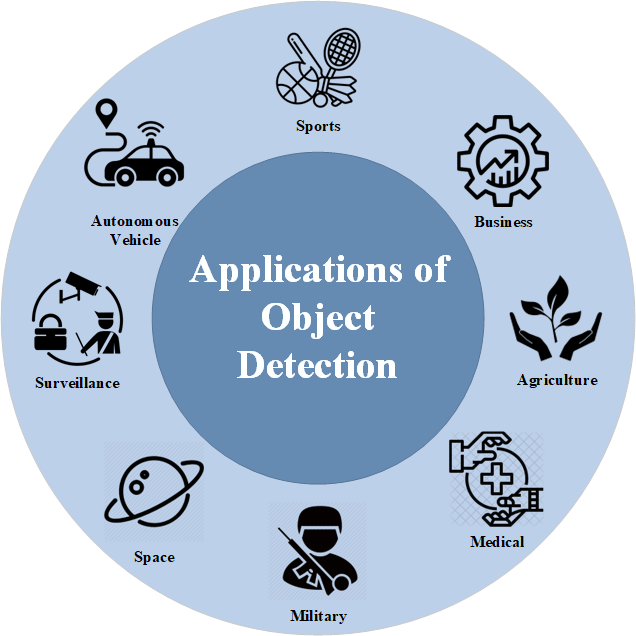
\includegraphics[width=0.5\textwidth]{images/Object Detection Application.png}
    \caption{Applications of Object Detection Methods}
  \end{figure}
\\\\
% This block inserts a figure displaying the applications of object detection methods.
% The '[h!]' option tells LaTeX to try and place the figure "here" (at the current location).
% '\centering' centers the figure horizontally on the page.
% The image file is inserted using '\includegraphics', and the 'width' option scales it to 30% of the page width.
% '\caption' adds a description below the figure.
%
Object detection has become an essential component in many real-world applications, including:
% This sentence introduces a list of real-world applications where object detection is crucial.
%
\begin{itemize}
  \item \textbf{Surveillance Systems and Public Safety:} Object detection is widely used in monitoring public spaces for security purposes, detecting potential threats or suspicious activities in real-time.
  \item \textbf{Autonomous Vehicles and Traffic Management:} In self-driving cars, object detection helps identify road elements such as pedestrians, vehicles, and traffic signs, enabling safe navigation and collision avoidance.
  \item \textbf{Robotics:} By incorporating object detection, robots can interact with their surroundings, such as grasping objects or navigating through obstacles.
  \item \textbf{Medical Imaging:} Object detection aids medical professionals in diagnosing diseases by identifying abnormalities such as tumors or lesions in medical images.
  \item \textbf{Industrial Automation:} Object detection plays a critical role in automating tasks like quality control, defect detection, and monitoring production lines in manufacturing industries.
  \\
\end{itemize}
% This block creates an itemized list of applications for object detection, with each application highlighted in bold.
% '\item' introduces each new item in the list.
% The double '\\' introduces extra spacing after the list.
%
% 1.2
{ \textbf{1.2 {Object Detection Methods}}}
\\
% This creates a new bolded heading for section "1.2 Object Detection Methods".
% The '\\' forces a line break after the title.
%
\begin{itemize}
  \item[\textbf{A.}] \textbf{Traditional Object Detection Methods}\\\\ 
  % This creates the first item in the list with a subheading "A. Traditional Object Detection Methods" in bold.
  % Double '\\' adds extra spacing before the list of methods.
  %  
  Earlier object detection approaches rely on hand-crafted features and image processing techniques. Notable traditional methods include:
  \begin{itemize}
    \item \textbf{Viola-Jones Algorithm:} Known for its speed and efficiency, this algorithm uses Haar-like features and a cascade classifier to detect objects, particularly faces.
    \item \textbf{Histogram of Oriented Gradients (HOG):} HOG works by analyzing the gradient orientations in localized portions of an image and is commonly used for pedestrian detection.
    \item \textbf{Deformable Parts Model (DPM):} DPM treats objects as collections of deformable parts, using a sliding window approach to detect objects based on part configurations.\\
  \end{itemize}
  % This nested list introduces traditional object detection methods (Viola-Jones, HOG, DPM), with brief descriptions of each. 
  % '\item' and '\textbf' are used to create each bolded item with corresponding details.
  % '\\' adds extra spacing before the list of methods.
  %
  \item[\textbf{B.}] \textbf{Deep Learning-Based Object Detection Methods}\\\\
  % This is another item in the list with a subheading "B. Deep Learning-Based Object Detection Methods" in bold.
  % Double '\\' adds extra spacing before the list of methods.
  %
  The advent of deep learning has revolutionized object detection by improving both accuracy and speed. Some notable deep learning-based methods are:
  \begin{itemize}
    \item \textbf{Region-Based Convolutional Neural Networks (R-CNN) Family:} The  R-CNN series, including Fast R-CNN and Faster R-CNN, uses a two-stage approach: generating region proposals for potential object locations and then classifying them using convolutional neural networks (CNNs).
    \item \textbf{Single Shot MultiBox Detector (SSD):} SSD is a single-stage object detector that divides the image into a grid and predicts both bounding boxes and class probabilities from multiple feature maps at different scales.
    \item \textbf{You Only Look Once (YOLO):} YOLO is a single-stage detector known for its ability to detect objects in real-time by predicting bounding boxes and class probabilities directly from the entire image in one pass.
  \end{itemize}
  % This nested list introduces deep learning-based object detection methods, such as R-CNN, SSD, and YOLO, with explanations.
  %
  \begin{figure}[h!]
    \centering
    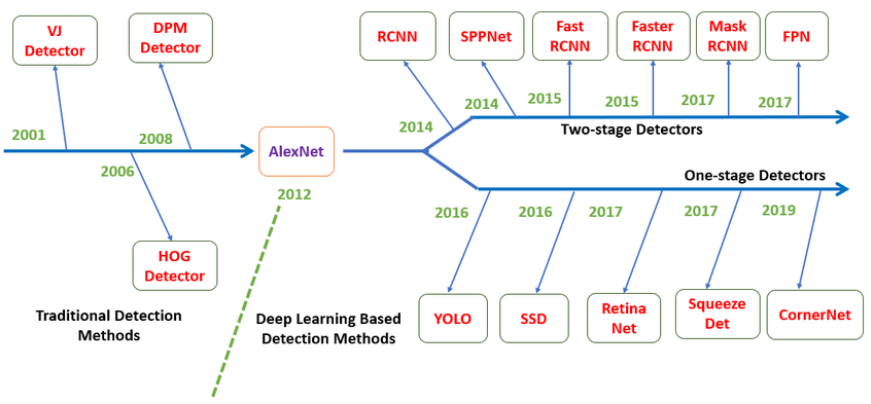
\includegraphics[width=0.7\textwidth]{images/Timeline.png}
    \caption{Timeline of Object Detection Methods}
    \label{fig:enter-label}
  \end{figure}
  % This block inserts a figure showing the timeline of object detection methods.
  % The 'label' command adds a reference to the figure that can be used elsewhere in the document. 
\end{itemize}
% This adds a new line and extra spacing after the list of methods.
%
% 1.3
{ \textbf{1.3 {YOLO (You Only Look Once)}}}\\\\
% This creates a new bolded heading for section "1.3 YOLO (You Only Look Once)".
% Double '\\' adds extra spacing after the section title.
%
YOLO is a family of single-stage object detection models recognized for their remarkable speed and accuracy. Unlike traditional two-stage detectors like Faster R-CNN, which first generate region proposals and then classify objects, YOLO simplifies the process by predicting bounding boxes and class probabilities in a single evaluation of the input image.
\\\newline
% This paragraph introduces YOLO and its key feature of using a single-stage detection process, compared to two-stage detectors like Faster R-CNN.
% '\\\newline' adds a new line and extra spacing after the paragraph.
%
\textbf{Key Features of YOLO: }
  \begin{itemize}
  \item \textbf{Unified Detection Process:} YOLO treats object detection as a single regression problem, directly predicting bounding boxes and class labels from the entire image in one step.
  \item \textbf{Real-Time Object Detection:} YOLO is optimized for speed, capable of performing real-time object detection with high frame rates, making it ideal for applications such as video analysis and autonomous systems.
  \item \textbf{End-to-End Optimization:} The entire YOLO pipeline is a single neural network, enabling end-to-end training and optimization, which contributes to improved detection performance.
  \item \textbf{High Accuracy:} YOLO models are known for their competitive accuracy on standard object detection benchmarks.
  \\
  \end{itemize}
% This block creates an itemized list of YOLO's key features, each of which is bolded and explained.
% '\item' is used to introduce each feature, and '\textbf' bolds the feature name.
% The '\\' adds a new line and extra spacing after the list.
%
% 1.4
{ \textbf{1.4 {Why YOLO}}}\\\\
% This creates a new bolded heading for section "1.4 Why YOLO".
% Double '\\' adds extra spacing after the section title.
%
YOLO has gained widespread popularity in computer vision due to its unique advantages over alternative object detection methods. Its combination of speed, accuracy, and simplicity makes it an attractive choice for a variety of applications, from real-time video analysis to autonomous systems.\\\\\\\\
% This paragraph explains why YOLO is popular and widely used, mentioning its advantages in terms of speed, accuracy, and simplicity.
% The double '\\\\\\\\' adds extra spacing before the following content.
%
\textbf{Advantages of YOLO: }
  \begin{itemize}
  \item \textbf{Speed:} YOLO’s single-stage architecture allows for real-time object detection with high frame rates, often outperforming two-stage detectors like Faster R-CNN in terms of speed. This makes YOLO highly suitable for applications requiring fast processing, such as video analysis and autonomous driving.
  \item \textbf{Accuracy:} YOLO delivers competitive accuracy on various benchmarks, making it reliable for a wide range of object detection tasks.
  \item \textbf{Generalization:} YOLO is capable of learning generalized representations of objects, improving its robustness and accuracy across different datasets.
  \item \textbf{Simplicity:} YOLO’s end-to-end design simplifies implementation, making it faster and easier than complex models like Faster R-CNN and more accurate than traditional methods like HOG and DPM.
  \end{itemize}
% This block creates an itemized list of the advantages of using YOLO, with each advantage highlighted in bold and followed by a description.
% '\item' introduces each new item, and '\textbf' is used for bold text.
%
YOLO stands out from other object detection methods by using a single-stage process, predicting bounding boxes and class probabilities in one step, unlike two-stage methods like Faster R-CNN. It is significantly faster, making it ideal for real-time applications.\\\\
% This paragraph summarizes how YOLO differs from other methods, emphasizing the single-stage process and its speed.
% The double '\\\\' adds extra spacing before the next content.
%
YOLO also uses anchor boxes to detect objects of varying sizes and generalizes better across different datasets compared to traditional hand-crafted feature methods. Its end-to-end training optimizes the entire network at once, making YOLO faster, simpler, and more adaptable than other object detection techniques.\\\\
% This paragraph further explains YOLO's use of anchor boxes for detecting objects of different sizes and highlights its generalization ability.
% The double '\\\\' adds extra spacing before the following figure.
%
\begin{figure}[h!]
    \centering
    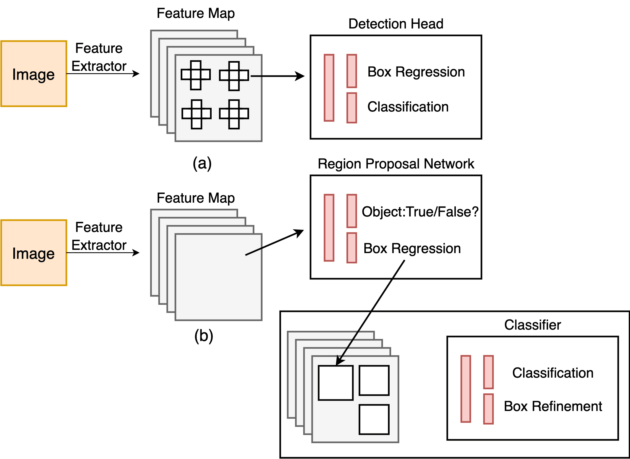
\includegraphics[width=0.7\textwidth]{images/1_vs_2 Stage.png}
    \caption{Single-Stage Detector vs Two-Stage Detector.}
\end{figure}
% This block inserts a figure that compares single-stage detectors (like YOLO) to two-stage detectors.
% '\centering' centers the figure horizontally on the page, and the 'width' option scales the image to 70% of the page width.
% '\caption' adds a description beneath the figure.
\\\\
% The double '\\\\' adds extra spacing before the next section.
%
% 1.5
{ \textbf{1.5 {How YOLO Works}}}\\\\
% This creates a new bolded heading for section "1.5 How YOLO Works".
% Double '\\' adds extra spacing after the section title.
%
YOLO is known for its innovative approach to object detection, offering both high speed and accuracy. Below is a detailed explanation of how the YOLO algorithm works:
% This sentence introduces the "How YOLO Works" section and mentions YOLO's key strengths of speed and accuracy.
%
\begin{enumerate}
  \item \textbf{Image Resizing and Grid Division:} YOLO first resizes the input image to a fixed size (e.g., 416x416) for standardization and efficiency. It then splits the image into an S x S grid, where each grid cell is responsible for detecting objects whose centers fall within it.
  % This is the first step in the YOLO process: resizing the image and dividing it into an SxS grid. The text explains how each grid cell detects objects based on their centers.
  %  
  \item \textbf{Bounding Boxes:} Each grid cell predicts B bounding boxes and confidence scores, indicating the likelihood that the box contains an object. Anchor boxes are used to define fixed aspect ratios and scales, enabling the model to better handle objects of varying shapes and sizes.
  % This step describes how each grid cell predicts bounding boxes and their confidence scores. The explanation also introduces anchor boxes for handling different object sizes and shapes.
  %
  \item \textbf{Prediction Generation:} For each bounding box, YOLO predicts:
   \begin{itemize}
  \item \textbf{Coordinates (x, y, w, h): } Center coordinates relative to the grid cell and dimensions relative to the image.
  % This explains that YOLO predicts the center coordinates (x, y) and dimensions (w, h) of each bounding box.
  %  
  \item \textbf{Confidence Score:} Represents the likelihood of an object being present and the accuracy of the box.
  % This defines the confidence score, which indicates how likely the bounding box contains an object and how accurate it is.
  %  
  \item \textbf{Class Probabilities:} Each grid cell predicts class probabilities, conditioned on containing an object.
  % This step mentions that class probabilities are predicted for each bounding box, but only if the grid cell contains an object.
   \end{itemize}
  % This is a nested itemized list within step 3, detailing the specific predictions YOLO makes for each bounding box.
  %
  \item \textbf{Non-Maximum Suppression (NMS):} NMS is used to eliminate duplicate detections, refining the results without significantly affecting performance.
  % The final step explains how Non-Maximum Suppression (NMS) is used to remove duplicate bounding boxes and ensure only the best detections are kept.
\end{enumerate}
% This block uses an enumerated list to explain the steps in the YOLO process: resizing and grid division, bounding box prediction, and non-maximum suppression.
%
\begin{figure}[h!]
    \centering
    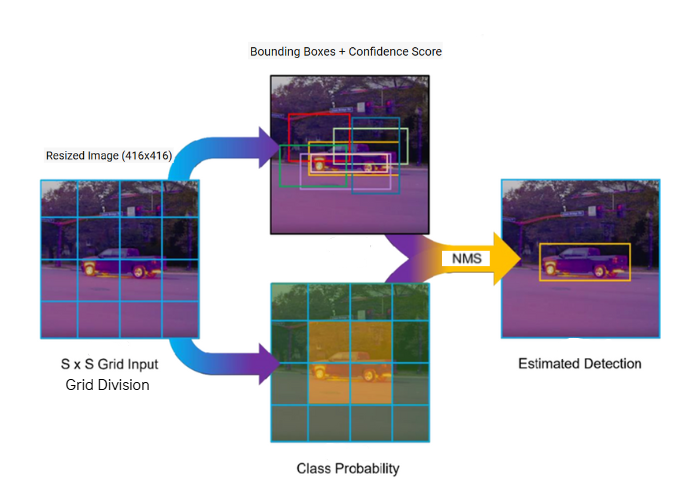
\includegraphics[width=0.7\textwidth]{images/Yolo Architecture.png}
    \caption{Working of YOLO}
\end{figure}
% This block inserts a figure showing the YOLO architecture.
% '\centering' centers the figure, and the 'width' option scales it to 70% of the page width.
% '\caption' adds a description below the figure.
%
% End of the chapter
%
%     % Includes the Introduction chapter
\chapter{Literature Survey}
%
% Paper 1
{ \textbf{[2.1] \underline{{ENHANCING REAL-TIME OBJECT DETECTION WITH YOLO ALGOR-}} \\ \underline{ITHM}}}\newline
\newline
%
This paper titled \textbf{"Enhancing real-time object detection with YOLO algorithm"}, authored by \textbf{Gudala Lavanya and Sagar Dhanraj Pande}, focuses on the advancements in real-time object detection through the YOLO (You Only Look Once) algorithm. Real-time object detection plays a vital role in areas like video surveillance, autonomous vehicles, and robotics. Traditional detection methods often require multiple passes over images, which increases the processing time. The YOLO algorithm, however, approaches object detection as a single-stage regression problem, predicting bounding boxes and class probabilities in one evaluation.\\\\
%
Due to its ability to detect objects in real-time with high accuracy, YOLO is highly regarded in the field of computer vision. The paper covers various versions of YOLO, highlighting their improvements in speed, accuracy, and handling of different object scales. YOLOv1 introduced a grid-based detection approach, while later versions incorporated anchor boxes, feature pyramids, and more sophisticated models like Darknet-53.\\\\
%
%
\textbf{The methodology of YOLO involves:}
\begin{enumerate}
  \item \textbf{Image Preprocessing:} The input image is resized to a uniform size.
  \item \textbf{Grid Division:} The image is divided into a grid, with each cell responsible for predicting bounding boxes and class probabilities.
  \item \textbf{Bounding Box Prediction:} The model predicts the center of each object within a grid cell and generates corresponding bounding boxes.
  \item \textbf{Class Label Assignment:} YOLO assigns class labels to detected objects based on confidence scores.
  \begin{itemize}
    \item \textbf{Confidence Score}: YOLO assigns a score to each bounding box, indicating the likelihood it contains an object.
    \item \textbf{Class Probabilities}: For each object, YOLO predicts probabilities for multiple classes (e.g., "car," "bus," "truck").
    \item \textbf{Class Label Assignment}: The class with the highest probability is assigned to the object.
    \begin{itemize}
       \item \textbf{Example}: If "car" = 0.8, "bus" = 0.6, and "truck" = 0.3, the object is labeled as "car."
    \end{itemize}
  \end{itemize}
  \item \textbf{Resolving Multiple Bounding Boxes:} Non-maximum suppression (NMS) is a fundamental technique YOLO employs to address this challenge.\\\\
  \textbf{Steps in NMS:}
  \begin{enumerate}
    \item Select the box with the highest confidence score, denoted as $\hat{c}$.
    \item Compute the Intersection over Union (IoU) between this box and all other boxes of the same class.
    \item Remove boxes with an IoU greater than a set threshold (typically 0.5).
    \item Repeat the process with the next highest confidence box until all boxes are processed.
    \item The remaining boxes are the final detections.
\end{enumerate}
\end{enumerate}
%
%
  \begin{figure}[h!]
    \centering
    
\includegraphics[width=0.5\textwidth]{images/IoU.png}
  \end{figure}
%  
% 
  \begin{figure}[h!]
    \centering
    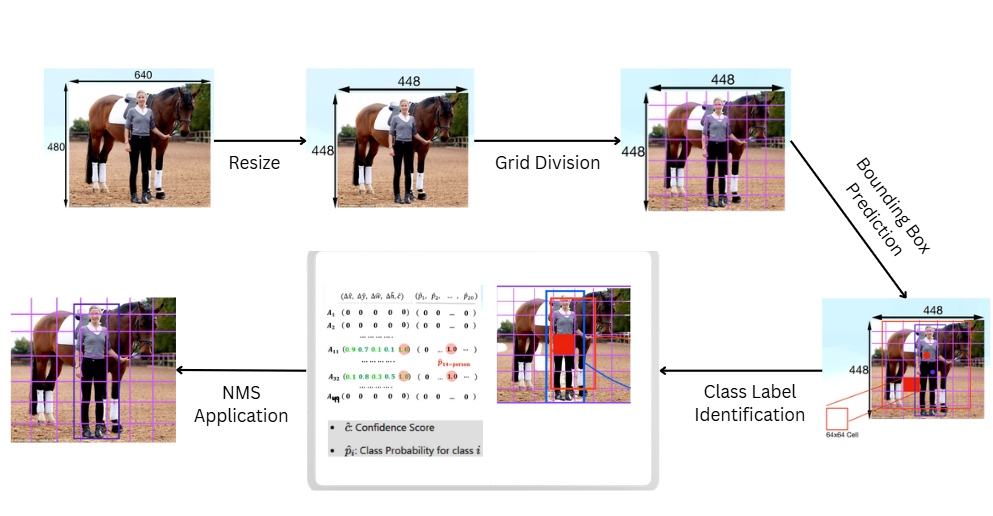
\includegraphics[width=1\textwidth]{images/Yolo Steps.png}
    \caption{Steps in YOLO}
  \end{figure}
%
%
The model was evaluated using standard datasets and achieved notable success due to its ability to process images in real-time, a key feature for applications that require immediate analysis of visual data.\\\\
%
The paper concludes by emphasizing YOLO's revolutionary impact on the field of real-time object detection. Its combination of speed and accuracy makes it a superior choice compared to traditional object detection methods. The continuous development across various versions (v1 to v8) has enhanced YOLO's ability to detect small objects, perform better on complex datasets, and improve overall detection efficiency.\\
%  
% 
\begin{figure}[h!]
    \centering
    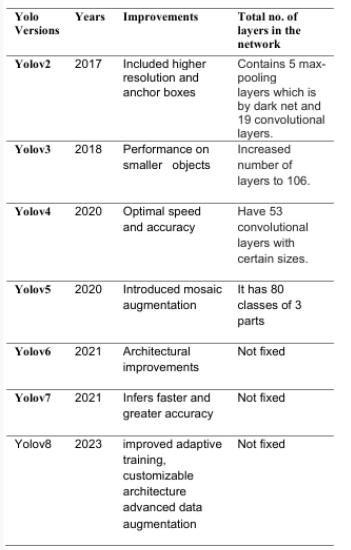
\includegraphics[width=0.8\textwidth]{images/YOLOv1 to YOLOv8.png}
    \caption{YOLO Versions Improvements Over Time}
\end{figure}\\\\
%
% Paper 2
{ \textbf{[2.2] \underline{IMPROVED YOLOv8 MODEL FOR A COMPREHENSIVE APPROACH TO } \\ \underline{OBJECT DETECTION AND DISTANCE ESTIMATION} }
\\\\
%
The paper titled \textbf{"Improved YOLOv8 Model for a Comprehensive Approach to Object Detection and Distance Estimation"}, authored by \textbf{Zu Jun Khow, Yi-Fei Tan, Hezerul Abdul Karim and Hairul Azhar Abdul Rashid}, proposes an enhanced object detection model called YOLOv8-CAW. This model builds on the YOLOv8 architecture and incorporates two key components: the Coordinate Attention (CA) module and the Wise-Intersection over Union (Wise-IoU) loss function, both of which work together to improve object detection accuracy and distance estimation.\\\\
%
The primary aim of the research is to address limitations in current models, especially for small object detection and distance estimation within the field of computer vision. The methodology focuses on integrating the CA module, which enhances the model’s focus on crucial regions of the image without significantly increasing its size. This attention mechanism captures positional information in both horizontal and vertical directions, resulting in more precise object localization. Additionally, the Wise-IoU loss function further enhances the training process by dynamically adjusting loss coefficients for high and low-quality samples, leading to more accurate bounding box predictions.\\\\
%
%  
% 
\begin{figure}[h!]
    \centering
    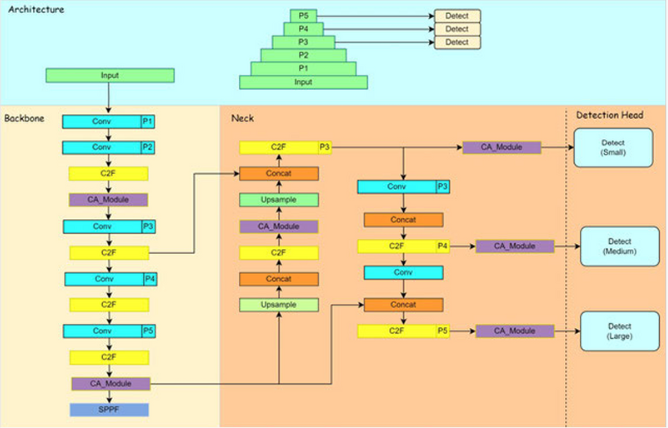
\includegraphics[width=0.7\textwidth]{images/YOLOv8 CAW Architecture.png}
    \caption{YOLOv8-CAW Model Architecture}
\end{figure}\\\\
%
%
Furthermore, the paper introduces a distance estimation technique, which calculates the distance between the camera and the detected object by comparing the real-world size of the object with its size in the captured image. This method achieves approximately 90\% accuracy based on experimental validation.\\\\
%
%
\textbf{The methodology consists of three core steps:}
\begin{enumerate}
  \item \textbf{Coordinate Attention (CA) Module:} The CA module in YOLOv8-CAW enhances localization accuracy and detection performance by focusing on relevant regions of the feature map without significantly increasing model size. This advanced attention mechanism embeds positional information into channel attention, allowing the network to concentrate on critical areas efficiently.
\\\\
\textbf{Key Features:}
\begin{itemize}
    \item \textbf{Positional Information Embedding:} Helps the model identify important object locations in the image.
    \item \textbf{Efficient Computation:} Processes the image in horizontal and vertical directions to improve relationships between features and enhance accuracy.
    \item \textbf{Directional Attention Maps:} Generates separate maps for horizontal and vertical focus, refining the detection process further.
\end{itemize}
%  
% 
\begin{figure}[h!]
    \centering
    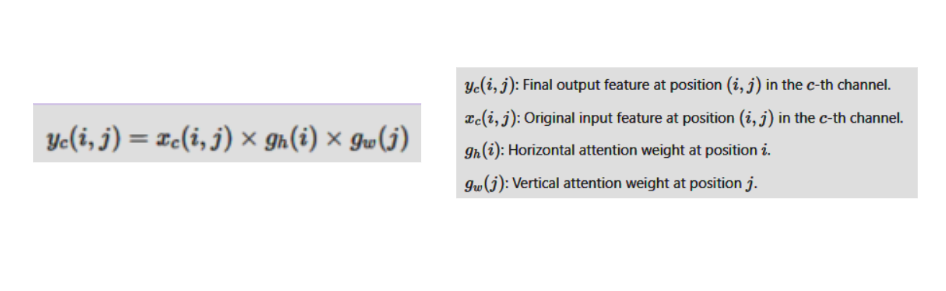
\includegraphics[width=1\textwidth]{images/CA Eqn.png}
\end{figure}
%
%
  \item \textbf{Wise-IoU Loss Function:} Improves the accuracy of bounding box predictions by focusing on the intersection between the predicted and ground truth bounding boxes.\\\\
  
  \textbf{A. Advantages of Wise-IoU over IoU:}
\begin{itemize}
    \item \textbf{Emphasizes Overlap:} Prioritizes intersection areas for more accurate predictions.
    \item \textbf{Robust to Small Overlaps:} Handles small overlaps better, reducing penalties for minor discrepancies.
    \item \textbf{Focus on Localization:} Adjusts loss based on spatial distribution, improving bounding box predictions.\\
\end{itemize}
\textbf{B. How Wise-IoU Works:}
\begin{itemize}
    \item Calculates the intersection area of predicted and ground truth boxes.
    \item Adjusts loss based on overlap degree, focusing on significant intersections.
    \item Encourages minimizing the distance between predicted and actual bounding boxes for better accuracy.
\end{itemize}
%  
% 
\begin{figure}[h!]
    \centering
    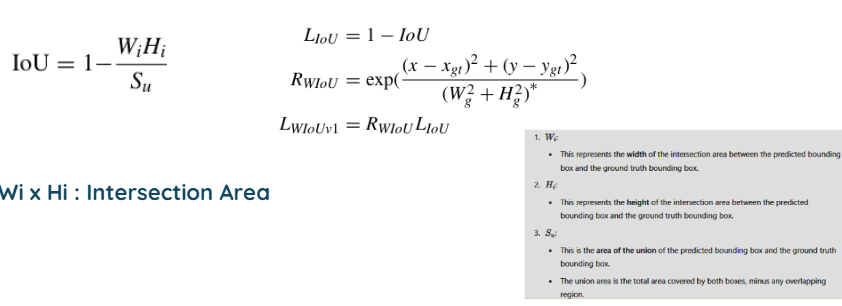
\includegraphics[width=1\textwidth]{images/WIoU Eqn.png}
\end{figure}
%
%
  \item \textbf{Distance Estimation Algorithm:} Uses the ratio calculation method to compare the average size of an object in the real world with its size in a captured image
\end{enumerate}
%  
% 
\begin{figure}[h!]
    \centering
    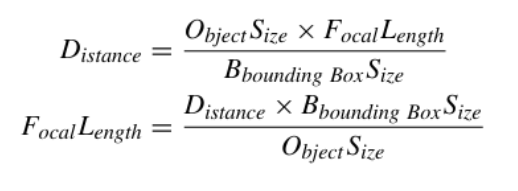
\includegraphics[width=0.5\textwidth]{images/Distance Estimation Eqn.png}
\end{figure}
%  
% 
\setlength{\fboxsep}{0pt} % Removes the padding around the image
\setlength{\fboxrule}{1pt} % Sets the thickness of the frame
%
%
\begin{figure}[h!]
    \centering
    \fbox{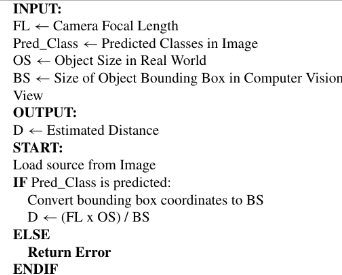
\includegraphics[width=0.5\textwidth]{images/Distance Estimation Algorithm.png}}
    \caption{Distance Estimation Algorithm}
\end{figure}
%
%
The model was tested on popular datasets like PASCAL VOC and MS-COCO, demonstrating improvements in recall, precision, and Mean Average Precision (mAP), with a particular focus on small object detection.\\\\
%
%
\begin{figure}[h!]
    \centering
    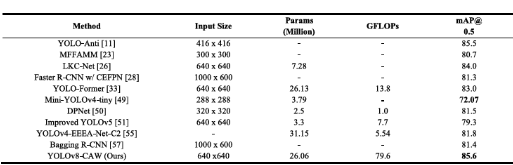
\includegraphics[width=1\textwidth]{images/YOLOv8-CAW vs Other Models.png}
    \caption{YOLOv8-CAW Model vs Other Model on Pascal VOC DataSet 2007}
\end{figure}
%
%
%
%
\begin{figure}[h!]
    \centering
    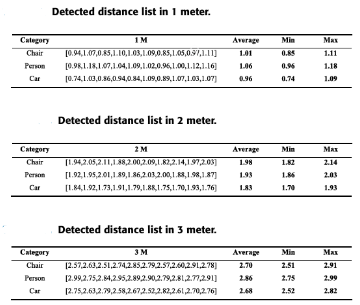
\includegraphics[width=0.8\textwidth]{images/Distance Estimation Result.png}
    \caption{Distance Estimation Result}
\end{figure}\\
%
%
% Paper 3
\noindent
{\textbf{[2.3] \underline{AUTOMATED VEHICLE COUNTING FROM PRE-RECORDED VIDEO } \\ \underline{USING YOLO OBJECT DETECTION MODEL}}}\\\\
%
The paper titled \textbf{"Automated vehicle counting from pre-recorded video using YOLO object detection model"}, authored by \textbf{Mishuk Majumder and Chester Wilmot}, introduces an automated method for vehicle counting from pre-recorded videos using the YOLOv3 (You Only Look Once) object detection model. Traffic monitoring is a critical component for urban planning, and traditional methods are often time-consuming and prone to errors. YOLOv3, with its ability to detect objects in real-time, provides a more efficient solution to this problem.\\\\
%
The paper's primary objective is to develop algorithms for detecting, tracking, and counting vehicles in pre-recorded videos. The dataset used in this study consists of video recordings from ten strip mall business sites located in Baton Rouge, Louisiana, recorded over two consecutive days.\\\\
%
%
\textbf{The methodology consists of the following steps:}
\begin{enumerate}
  \item \textbf{Data Collection and Pre-processing:} Videos were collected and pre-processed, including frame extraction and resizing for uniformity.
  \item \textbf{YOLO Version Selection:} YOLOv3 was chosen due to its balance between speed and accuracy, making it ideal for real-time detection.
  \item \textbf{Conversion to TensorFlow:} The YOLO weight file, originally in C/C++, was converted to the TensorFlow API to be used in Python. Python was preferred for its flexibility and ease of use in the project.
  \item \textbf{Setup:} The necessary video files were prepared in .mp4 format and uploaded into the system. Relevant settings, including the YOLO model configuration, video file location, and system resources such as available GPUs, were specified. The system was then checked and prepared for vehicle detection.
  \begin{itemize}
    \item \textbf{YOLO Model Settings}: Specify the location of the YOLO weight file, configure model settings (e.g., detection thresholds), and check available GPUs for processing.
    \item \textbf{Video File Settings}: Configure the video file name and its location for vehicle detection. Ensure the video is in \texttt{.mp4} format.
    \item \textbf{Prepare Video}: Convert the video files to \texttt{.mp4} if necessary and merge multiple video files if needed, as the program processes only one file at a time.
    \item \textbf{Upload Video}: Drag and drop the \texttt{.mp4} video into the input section. Enter the video name (excluding the \texttt{.mp4} extension) into the program.
    \item \textbf{Check and Process}: Run the program to verify the input files and settings. Once verified, the vehicle detection process can begin.
\end{itemize}
  \item \textbf{Reference Line Drawing and Vehicle Detection:} Reference lines were manually drawn on video frames as allowed by the algorithm to mark areas for vehicle detection. YOLOv3 was then used to generate bounding boxes around the detected vehicles.
  \item \textbf{Vehicle Tracking:} Vehicles were tracked across multiple frames using the Kalman Box Tracker, which compared pixel values between frames to keep track of the vehicles' locations. Each detected vehicle was assigned a unique ID for identification.
  \begin{itemize}
    \item \textbf{Tracking Objects}: To track vehicles across thousands of video frames, the program compares each frame with the previous one using pixel differences.
    \item \textbf{Kalman Box Tracker}: This algorithm tracks bounding boxes by checking for similarities in pixel values across frames, updating and memorizing the vehicle’s bounding boxes.
    \item \textbf{Identification and Display}: Each detected vehicle is assigned a unique numeric ID. Rectangles are drawn around tracked objects, and a dotted centerline is used to aid vehicle counting.
\end{itemize}
  \item \textbf{Vehicle Counting:} The direction of vehicle movement was determined based on whether it crossed the reference line from left to right (entry) or right to left (exit). Counters for both directions were maintained using custom algorithms.
\begin{itemize}
    \item \textbf{Counting Directions}: The direction of vehicle movement is determined by whether the center point of the bounding box (BB) crosses the reference line:
    \begin{itemize}
        \item \textbf{Entry Count (L2R)}: Vehicles crossing from left to right (L2R) are counted as entering.
        \item \textbf{Exit Count (R2L)}: Vehicles crossing from right to left (R2L) are counted as exiting.
    \end{itemize}
    \item \textbf{Functions for Counting}:
    \begin{itemize}
        \item \texttt{leftToRight\_counter}: Tracks and counts vehicles entering from the left.
        \item \texttt{rightToLeft\_counter}: Tracks and counts vehicles exiting from the right.
    \end{itemize}
\end{itemize}
\item \textbf{Output:} The program outputs vehicle counts in both a spreadsheet and on-screen, with real-time adjustments for accurate tracking and customizable time intervals.
\begin{itemize}
    \item \textbf{Output Format}: The program generates a spreadsheet displaying vehicle counts for each direction (entry or exit) over a flexible time interval.
    \item \textbf{Time Interval Adjustment}: YOLO calculates the number of frames and the processing time per frame to match real-time intervals. The YOLO time interval is adjusted accordingly for accurate counts.
    \item \textbf{Display}: Vehicle counts are displayed on the computer screen and in the spreadsheet, with detailed examples provided (e.g., entry and exit counts at locations such as strip malls).
\end{itemize}
\end{enumerate}
%
%
\begin{figure}[h!]
    \centering
    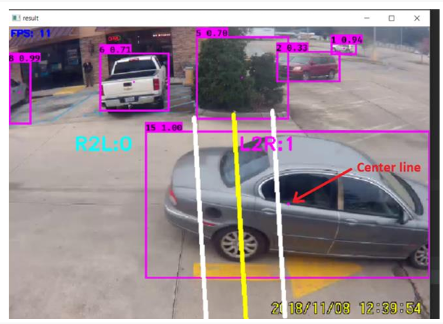
\includegraphics[width=0.4\textwidth]{images/Paper 3 Algorithm Implementation.png}
    \caption{YOLO-Based Vehicle Detection with Center Line and Direction Indicators}
\end{figure}
%
%
\begin{figure}[h!]
    \centering
    \fbox{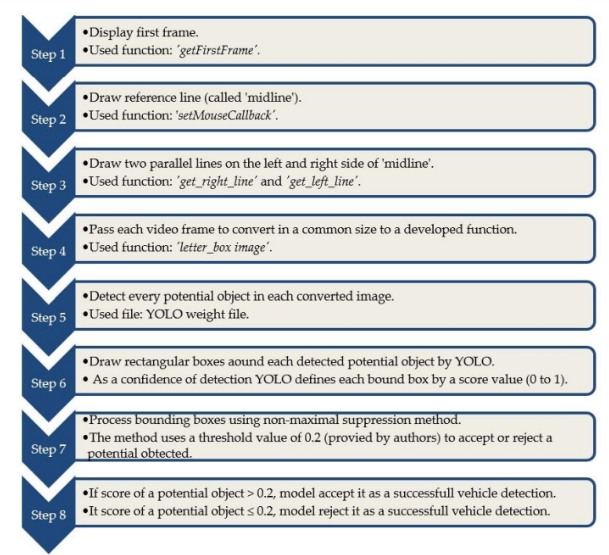
\includegraphics[width=0.8\textwidth]{images/Paper 3 Algorithm.png}}
    \caption{Step-by-Step Process for Vehicle Detection Using YOLO and Line Detection}
\end{figure}
%
%
The results were outputed in a spreadsheet format that included vehicle counts over specified time intervals. The results were displayed in real-time on the screen as well as logged in the spreadsheet, with counts showing vehicles entering and exiting various locations such as strip malls. This study demonstrates the effectiveness of YOLOv3 for automating vehicle counting, providing a fast and reliable solution for traffic monitoring and urban planning purposes.\\\\
%
%
\begin{figure}[h!]
    \centering
    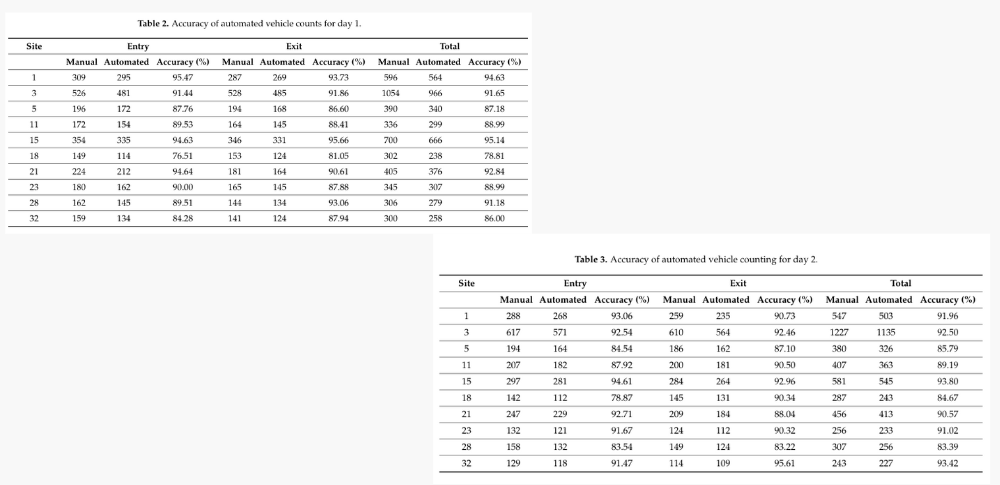
\includegraphics[width=0.8\textwidth]{images/Paper 3 Result.png}
    \caption{Accuracy of Manual vs Automated Vehicle Counts for Two Days}
\end{figure}
%
%
\newpage
\noindent
% Paper 4
{\textbf{[2.4] \underline{MODIFIED YOLO MODULE FOR EFFICIENT OBJECT TRACKING IN} \\ \underline{A VIDEO}}}\\\\
%
The paper titled \textbf{"Modified YOLO Module for Efficient Object Tracking"},authored by \textbf{Varsha Kshirsagar, Raghavendra Bhalerao, and Manish Chaturvedi}, proposes enhancements to the YOLO (You Only Look Once) algorithm to improve object tracking accuracy in video sequences. It addresses the challenges posed by fluctuations in confidence scores and misclassification of objects between consecutive frames, which often affect tracking and counting tasks, especially in complex environments like traffic monitoring.\\\\
%
The original YOLO algorithm is widely recognized for its real-time object detection capabilities. However, it struggles with sudden drops in confidence scores across frames, leading to incorrect object classification and tracking inaccuracies. To overcome these limitations, the authors propose a modification that integrates RANSAC (Random Sample Consensus) algorithm and linear interpolation to smooth out confidence score fluctuations and improve overall tracking performance.
%
%
\begin{figure}[h!]
    \centering
    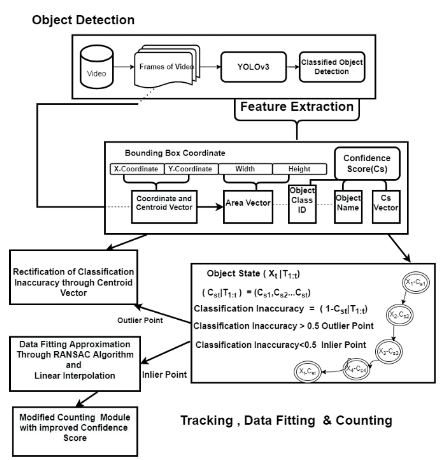
\includegraphics[width=0.8\textwidth]{images/Paper 4 Architecture.png}
    \caption{Enhanced Object Detection and Tracking Framework}
\end{figure}
%
%
\newpage
\noindent
\textbf{The methodology presented in the paper involves several key steps:}
\begin{enumerate}
  \item \textbf{Object Detection Using YOLO:} The YOLO algorithm is employed for object detection across video frames. It uses bounding boxes, object class, and confidence scores to detect
 objects, particularly vehicles, in each frame
  \begin{itemize}
    \item \textbf{YOLO's Strength in Single Frames:} YOLO's ability to perform well on single frames makes it particularly suitable for detecting objects accurately in each frame.
    \item \textbf{YOLOv3 for Vehicle Detection:} YOLOv3 is specifically used due to its effectiveness in detecting vehicles, making it ideal for tasks focused on identifying cars, buses, and other vehicles.
  \end{itemize}

 \item \textbf{Feature Extraction:} Critical features such as object size, centroid coordinates, and confidence scores are extracted from the YOLO output. These features are essential for accurately tracking objects across frames.
  \begin{itemize}
      \item \textbf{Key Features from YOLOv3:} YOLOv3 uses bounding box dimensions, centroid coordinates, object class, and confidence score for object detection and tracking.
      \item \textbf{Importance of Multiple Features:} Combining features enhances tracking accuracy, especially when some features are unreliable in certain frames (e.g., due to occlusion).
      \item \textbf{Tracking Parameters:} The extracted parameters, along with the centroid smooth curve of the area, are utilized to track particular targets throughout the video.
  \end{itemize}
 \item \textbf{Outlier Rejection and Data Fitting:} Outliers, or frames with drastic changes in confidence scores or misclassification, are identified and rejected using the \textbf{RANSAC} algorithm. To ensure a smoother confidence score trajectory across frames and maintain continuity in object tracking (Data Fitting), \textbf{Linear Interpolation} is applied to fill gaps caused by the rejected outliers.
 \begin{itemize}
    \item \textbf{Outlier:} Data points that significantly deviate from the norm; in this case, frames where the confidence score drops or object class changes unexpectedly.
    \item \textbf{Identification:} Outliers are detected when confidence scores fall below a threshold or show abrupt variations.
    \item \textbf{Confidence Score (Cs):}
    \begin{itemize}
        \item \textbf{Definition:} Measures the certainty of object detection.
        \item \textbf{Formula:} 
        \[
        \text{Confidence Score} = Pr(\text{object}) \times IOU
        \]
        \item \textbf{Pr(object):} Probability of the object class \( 0 < Pr < 1 \)
        \item \textbf{IOU (Intersection over Union):} Overlap measure \( 0 < IOU < 1 \)
        \item \textbf{Max Value:} 1 (100\% confidence)
    \end{itemize}
    \item \textbf{Handling Classification Inaccuracy:}
    \begin{itemize}
        \item \textbf{Inaccuracy Formula:}
        \[
        1 = \text{ConfidenceScore} + \text{ClassificationInaccuracy}
        \]
        \item \textbf{Threshold Handling:} 
        \begin{itemize}
            \item If Inaccuracy \( > 0.5 \), retain previous class ID:
            \[
            \text{Class id}(n) = \text{Class id}(n-1)
            \]
            \item Replace outlier points with 0.
        \end{itemize}
    \end{itemize}
    \item \textbf{Tracking Improvements:}
    \begin{itemize}
        \item \textbf{RANSAC Algorithm:} Smooths tracking by identifying inliers and correcting outliers.
        \item \textbf{Linear Interpolation:} Fills gaps in confidence score data.
        \item \textbf{Area Consistency:} Object area should be 80-90\% of the previous frame’s area to maintain tracking.
    \end{itemize}
\end{itemize}

 \item \textbf{Object Tracking and Counting:} A and B represents vehicle and marker line, index vectors of these two vectors are ia and ib.
%
%
\begin{figure}[h!]
    \centering
    \fbox{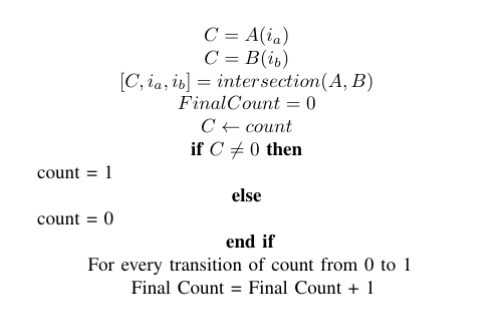
\includegraphics[width=0.8\textwidth]{images/Paper 4 Algorithm.png}}
    \caption{Object Counting Algorithm: Intersection-Based Counting Logic}
\end{figure}
%
%
\end{enumerate}
%
%
\textbf{RANSAC Algorithm}
\begin{itemize}
    \item The RANSAC algorithm minimizes the effect of outlier points and provides the best-fitted model with inlier points.
    \item The algorithm proposes a model from the extracted data, accounting for variations in confidence scores due to factors such as shadow and occlusion.
    \item RANSAC assists in finding a perfect curve from the extracted confidence score data obtained through YOLO.
\end{itemize}
%
%
\begin{figure}[h!]
    \centering
    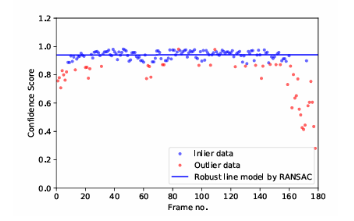
\includegraphics[width=0.8\textwidth]{images/RANSAC Outlier Rejection.png}
    \caption{Outlier Rejection by RANSAC algorithm}
\end{figure}
%
%
\textbf{Linear Interpolation Algorithm}
\begin{itemize}
    \item Linear interpolation can identify the nearest point from the collected information of outlier and inlier points from the RANSAC approximation.
    \item Initially, outlier points are replaced by zero.
    \item Afterwards, linear interpolation is used to fill these zeros with appropriate values.
\end{itemize}
%
%
\begin{figure}[h!]
    \centering
    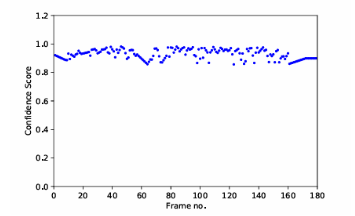
\includegraphics[width=0.8\textwidth]{images/Linear Interpolation.png}
    \caption{Track approximation by RANSAC and Linear Interpolation.}
\end{figure}
%
%
The modified YOLO module was tested on custom traffic datasets and demonstrated significant improvements in object tracking and classification accuracy. Vehicle counting accuracy increased from 66\% to 87\%, and the overall classification accuracy ranged between 94\% and 96\%. This makes the proposed method highly effective for real-time applications, such as traffic monitoring and autonomous vehicle systems.\\\\
%
The integration of RANSAC and linear interpolation into the YOLO framework addresses key challenges in object tracking and classification, offering a robust solution for real-time applications. By maintaining consistent confidence scores and correcting misclassified frames, the modified YOLO module significantly improves both object tracking and counting accuracy.This enhancement makes it a valuable tool for video analysis tasks, especially in environments like traffic monitoring, where object tracking consistency is crucial.\\\\
%
%
%
%
\begin{figure}[h!]
    \centering
    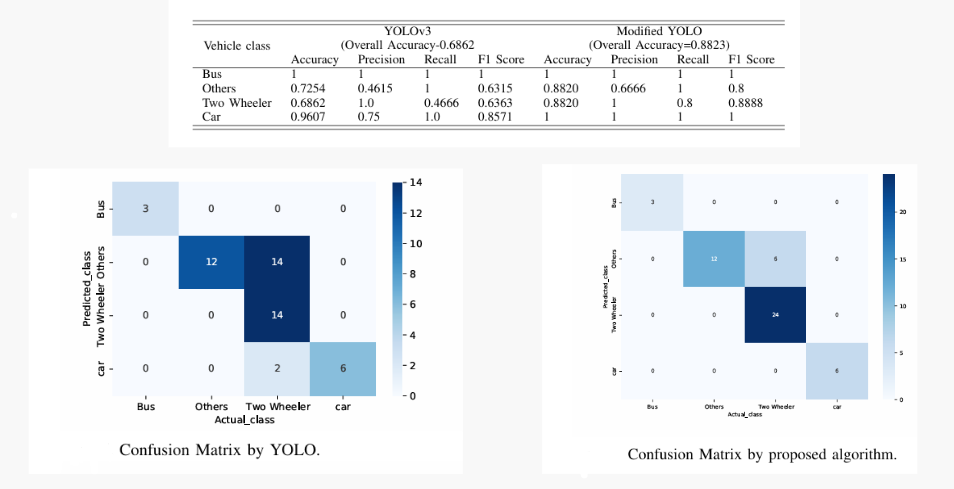
\includegraphics[width=1\textwidth]{images/Comparison of YOLOv3 and Modified YOLO Performance.png}
    \caption{Comparison of YOLOv3 \& Modified YOLO with RANSAC and Linear Interpolation}
\end{figure}
%
%  % Includes the Literature Survey chapter
\chapter{Comparison}
%
% 3.1
{ \textbf{3.1 {YOLO vs Traditional and Deep-Learning Object Detection Methods}}}\newline
\newline
%
Object detection has evolved from traditional methods like HOG+SVM and Haar Cascades to advanced deep learning models such as YOLO, Faster R-CNN, and EfficientDet. Traditional approaches struggle in complex environments, while deep learning models provide superior speed and accuracy. Among them, YOLO stands out for its real-time performance, making it ideal for applications like autonomous driving and surveillance, where speed is critical.\\\\
%
%
  \begin{figure}[h!]
    \centering
    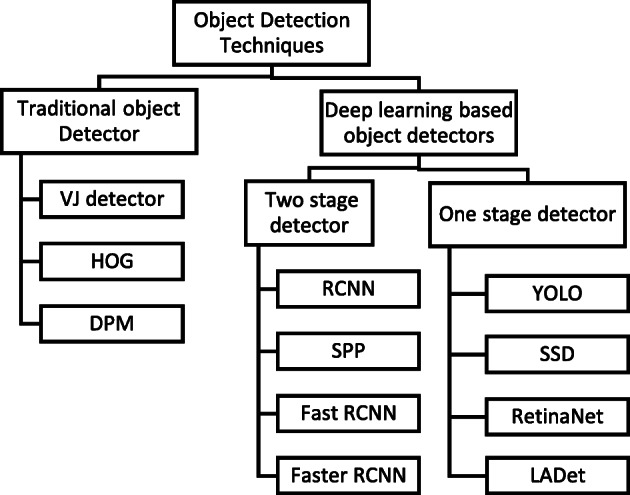
\includegraphics[width=0.5\textwidth]{images/Object Detection Techniques.png}
    \caption{Object Detection Techniques}
    \label{fig:enter-label}
  \end{figure}
\\\\\\
%
%
YOLO surpasses traditional methods like HOG+SVM and Haar Cascades in every aspect. Traditional methods rely on hand-engineered features, which are less robust in complex environments. YOLO’s ability to learn features directly from data makes it much more adaptable and accurate in real-world scenarios. Traditional methods also lack the capability to process multiple objects efficiently and are unsuitable for tasks requiring real-time detection, unlike YOLO, which excels in these areas.\\
%
% Table 1
\begin{table}[ht]
\centering
\caption{YOLO vs Traditional Methods}
\vspace{0.3cm} 
\begin{tabular}{|l|l|l|p{4.5cm}|p{4.5cm}|}
\hline
\textbf{Method}       & \textbf{Speed} & \textbf{Accuracy} & \textbf{Strengths}                                 & \textbf{Weaknesses}                               \\ \hline
\textbf{YOLO}         & 30-45 FPS      & High             & Learns features automatically, real-time capable  & Struggles with small objects                     \\ \hline
\textbf{HOG+SVM}      & Slow           & Low              & Simplicity, low computational cost                & Fails in complex environments                    \\ \hline
\textbf{Haar Cascades} & Moderate       & Low              & Efficient for simple tasks                        & Limited object variety, low accuracy             \\ \hline
\end{tabular}
\label{tab:yolo_vs_traditional}
\end{table}
\\\\
%
%
While methods like Faster R-CNN, RetinaNet, and EfficientDet offer higher accuracy, YOLO remains the leading choice for real-time object detection due to its exceptional speed. YOLO processes the entire image in a single forward pass, eliminating the need for region proposals or multi-scale feature extraction, which slows down other methods. This efficiency, combined with a strong balance between speed and accuracy, makes YOLO the preferred method for applications like autonomous driving, surveillance, and robotics, where every millisecond counts. combine this with above one.
%
% Table 2
\begin{table}[H]
\centering
\caption{Comparison of YOLO with Other Deep Learning Methods}
\vspace{0.3cm} 
\begin{tabular}{|l|c|c|p{3.5cm}|p{3.5cm}|}
\hline
\textbf{Method}       & \textbf{Speed}         & \textbf{Accuracy} & \textbf{Strengths}                       & \textbf{Weaknesses}                          \\ \hline
\textbf{YOLO}         & 30-45 FPS              & High              & Real-time detection                      & Struggles with small objects                 \\ \hline
\textbf{Faster R-CNN} & Moderate (10 FPS)      & Very High         & High accuracy, good for complex scenes   & Slower than YOLO due to region proposals     \\ \hline
\textbf{RetinaNet}    & Moderate (5-15 FPS)    & High              & Focuses on dense object detection        & More complex architecture, slower inference  \\ \hline
\textbf{EfficientDet} & Moderate               & Very High         & Efficient scaling, high accuracy         & Requires more computational resources        \\ \hline
\textbf{SSD}          & 20-40 FPS              & High              & Fast detection, suitable for real-time applications & Struggles with detecting smaller objects     \\ \hline
\textbf{Mask R-CNN}   & Slow (5-10 FPS)        & Very High         & Can detect objects and generate segmentation masks & Slower due to additional segmentation steps  \\ \hline
\textbf{Cascade R-CNN}& Slow (5-10 FPS)        & Very High         & High accuracy, especially for detecting objects at different scales & Computationally expensive, slow inference    \\ \hline
\end{tabular}
\label{tab:yolo_vs_other_methods}
\end{table}
%
% 
\begin{figure}[H]
    \centering
    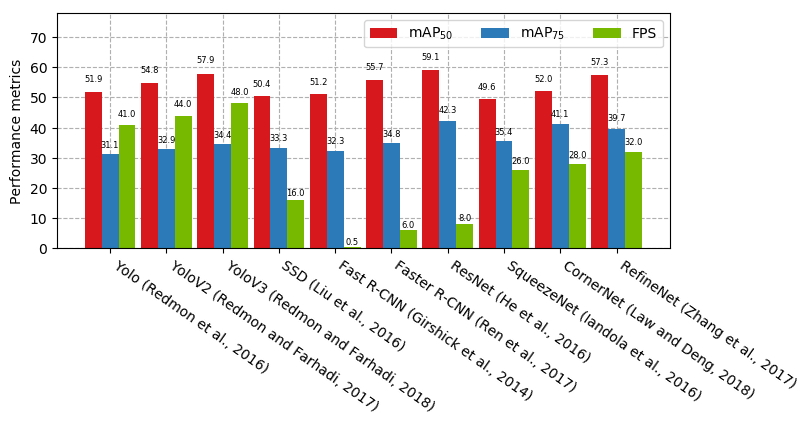
\includegraphics[width=0.9\textwidth]{images/Yolo vs Other Models.png}
    \caption{Performance Metrics of Object Detection Techniques on Pascal VOC 2012 Dataset}
    \label{fig:performance_metrics}
\end{figure}
%
% Section 3.2
\section*{3.2 YOLOv1 - YOLOv8}
The YOLO (You Only Look Once) object detection algorithm, introduced by Joseph Redmon in 2016, revolutionized object detection by offering a real-time approach with high accuracy and speed. Unlike traditional methods, YOLO treats object detection as a single regression problem, predicting bounding boxes and class probabilities from full images. Over the years, YOLO has undergone significant evolution. YOLOv1 pioneered real-time detection but struggled with small objects. YOLOv2 introduced anchor boxes and batch normalization for better accuracy, while YOLOv3 improved detection using a deeper network and multi-scale predictions. YOLOv4 introduced advanced techniques like PANet and self-adversarial training, further boosting performance. YOLOv5 gained popularity for its ease of use and mobile optimization, while YOLOv6 and YOLOv7 further refined speed and accuracy. YOLOv8, the latest version, offers the most advanced architecture, excelling in both speed and accuracy across multiple tasks. Each version allows customization and fine-tuning for specific applications, making YOLO highly versatile in various object detection tasks.
%
%
  \begin{figure}[h!]
    \centering
    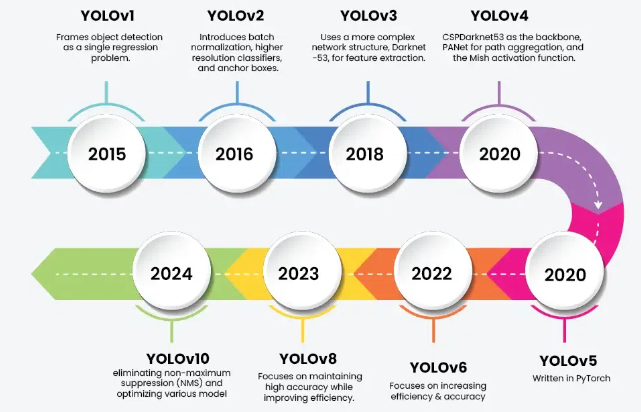
\includegraphics[width=0.5\textwidth]{images/Yolo Timeline.png}
    \caption{YOLO Timeline}
    \label{fig:enter-label}
  \end{figure}\\
%
%
YOLO versions can be easily modified and customized for specific tasks through transfer learning and fine-tuning on custom datasets. Users can adjust anchor box dimensions, change the number of output classes, or alter the architecture by adding or removing layers, depending on the use case. Additionally, modifications can include changes to the architecture (CA) and loss functions to enhance performance (Eg: YOLOv8-CAW model). The introduction of algorithms designed to overcome specific drawbacks found in previous variants further improves their efficacy (Eg: Outlier Rejection and Linear Interpolation). The simplicity of the YOLO architecture also allows for seamless integration with other algorithms (e.g., attention mechanisms, R-CNN features) for enhanced performance. 
%
% Table 3
\begin{table}[ht]
\centering
\caption{Comparison of YOLO Versions}
\vspace{5pt} 
\begin{tabular}{|p{1.8cm}|p{1.2cm}|p{2.5cm}|p{1.8cm}|p{1.8cm}|p{5.5cm}|} 
\hline
\textbf{Version} & \textbf{Year} & \textbf{Backbone} & \textbf{Speed (FPS)} & \textbf{Accuracy \small{(mAP@50)}} & \textbf{Key Features} \\ \hline
YOLOv1  & 2016 & Custom CNN       & 45 FPS   & 63.4\%  & Single-scale detection, simple architecture \\ \hline
YOLOv2  & 2017 & Darknet-19       & 67 FPS   & 76.8\%  & Anchor boxes, batch normalization, multi-scale detection \\ \hline
YOLOv3  & 2018 & Darknet-53       & 30 FPS   & 78.6\%  & Residual blocks, multi-scale predictions, feature pyramids \\ \hline
YOLOv4  & 2020 & CSPDarknet53     & 60 FPS   & 89.7\%  & PANet, SAT, advanced data augmentation, efficient backbone \\ \hline
YOLOv5  & 2020 & Focus + CSPNet   & 140 FPS  & 88.0\%  & PyTorch implementation, easy deployment, mobile-friendly \\ \hline
YOLOv6  & 2022 & EfficientRep     & 150+ FPS & 89.6\%  & EfficientRep backbone, optimized for GPUs, better quantization \\ \hline
YOLOv7  & 2022 & E-ELAN           & 160 FPS  & 90.2\%  & Model re-parameterization, versatile architecture \\ \hline
YOLOv8  & 2023 & Ultralytics Backbone & 170 FPS  & 91.0\%  & Advanced architecture, improved support for multiple tasks \\ \hline
\end{tabular}
\label{tab:yolo_versions}
\end{table}
%
%
  \begin{figure}[h!]
    \centering
    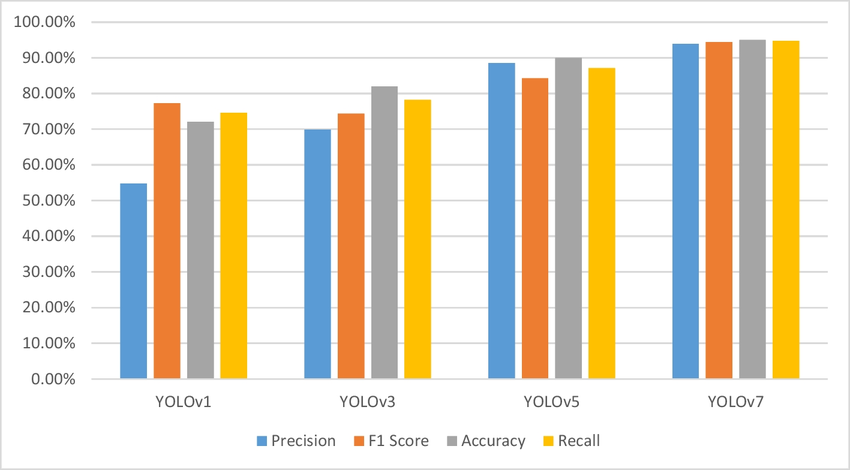
\includegraphics[width=0.7\textwidth]{images/Yolo Variants Performance Metrics.png}
    \caption{YOLO Variants Performance Metrics}
    \label{fig:enter-label}
  \end{figure}
%
%      % Includes the Comparison chapter
\chapter{Conclusion}
Add your conclusion content here.
      % Includes the Conclusion chapter

% Stop indenting after chapters (for sections like Bibliography or Appendix)
\addtocontents{toc}{\protect\setlength{\cftchapindent}{0em}}  % Reset indent for subsequent entries

% Bibliography Page
\begin{thebibliography}{00}
% Begins the bibliography environment. The parameter {00} sets the width for the references.
%
%
% Reference 1
\bibitem{b1} G. Lavanya and S. D. Pande, ``Enhancing real-time object detection with YOLO algorithm,'' \textit{EAI Endorsed Transactions on Internet of Things}, vol. 10, 2023.
% Cites the first reference with authors, title, journal name, volume, and year.
%
% Reference 2
\bibitem{b2} Z. J. Khow, Y. F. Tan, H. A. Karim, and H. A. A. Rashid, ``Improved YOLOv8 model for a comprehensive approach to object detection and distance estimation,'' \textit{IEEE Access}, vol. 12, pp. 1--10, 2024.
% Cites the second reference with authors, title, journal name, volume, page range, and year.
%
% Reference 3
\bibitem{b3} M. Majumder and C. Wilmot, ``Automated vehicle counting from pre-recorded video using You Only Look Once (YOLO) object detection model,'' \textit{Journal of Imaging}, vol. 9, p. 456, 2023.
% Cites the third reference with authors, title, journal name, volume, and page number.
%
% Reference 4
\bibitem{b4} V. K. Deshpande, R. Bhalerao, and M. Chaturvedi, ``Modified YOLO module for efficient object tracking,'' \textit{IEEE Latin America Transactions}, vol. 21, pp. 123--134, 2023.
% Cites the fourth reference with authors, title, journal name, volume, page range, and year.
%
% Reference 5
\bibitem{b5} J. Redmon, S. Divvala, R. Girshick, and A. Farhadi, ``You Only Look Once: Unified, real-time object detection,'' \textit{Proceedings of the IEEE Conference on Computer Vision and Pattern Recognition (CVPR)}, pp. 779--788, 2016.
% Cites the fifth reference with authors, title, conference name, page range, and year.
%
% Reference 6
\bibitem{b6} M. Hussain, ``YOLOv1 to v8: Unveiling each variant—a comprehensive review of YOLO,'' \textit{Journal of Artificial Intelligence Research}, vol. 18, pp. 123--145, 2024.
% Cites the sixth reference with the author's name, title, journal name, volume, page range, and year.
%
% Reference 7
\bibitem{b7} Q. Liu, H. Ye, S. Wang, and Z. Xu, “YOLOv8-CB: Dense Pedestrian Detection Algorithm Based on In-Vehicle Camera,” \textit{Electronics}, vol. 13, no. 1, p. 236, 2024.
% Cites the seventh reference with authors, title, journal name, volume, issue number, and page number.
%
%
\end{thebibliography}
% Ends the bibliography environment.
%
%
\addcontentsline{toc}{chapter}{Bibliography}
% Includes the Bibliography and adds it to the table of contents.

% Appendix A Page
\prefacesection{Appendix A: Presentation Slides}
% Creates a section titled "Appendix A: Presentation Slides" in the preface.
%
%
% Displaying the first two slides as an image.
\begin{figure}[h!]
    \centering
    % Centers the image on the page.
    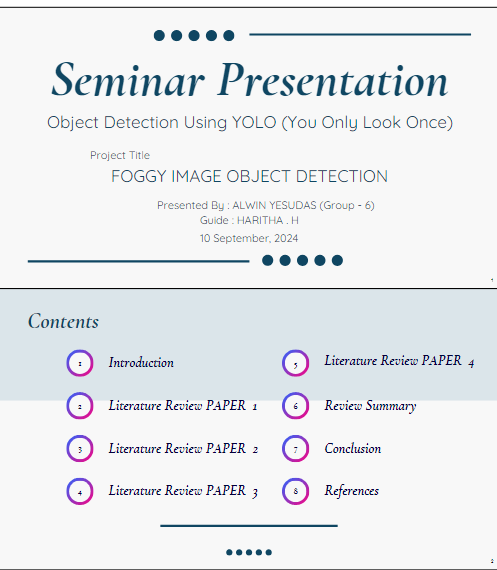
\includegraphics[width=1\textwidth]{images/Slide 1-2.png}
    % Includes an image file called "Slide 1-2.png" from the 'images' folder.
    % The image is scaled to the full width of the text area (\textwidth).
\end{figure}
% Ends the figure environment that contains the first two slides.
%
%
%
% Including slides 3 to 44 as a PDF with 2 slides per page.
\includepdf[nup=1x2, pages={3-44}, frame, pagecommand={\thispagestyle{plain}}]{pdfs/Seminar Presentation.pdf}
% \thispagestyle{plain}   ensures the page number is displayed
% Inserts pages 3 to 44 from a PDF file called "Seminar Presentation.pdf" located in the 'pdfs' folder.
% The option nup=1x2 places 2 slides per page in a 1-row, 2-column layout.
% The 'frame' option draws a border around each slide.
%
% End of the chapter
%
%
% Includes Appendix A.

% Appendix B Page
\prefacesection{Appendix B: Reference Papers}
% Creates a section titled "Appendix B: Reference Papers" for displaying the reference papers.
%
%
% Paper 1
\vspace{-5mm}
% Adds vertical space of -5mm, reducing the space between the title and the first paper.
\textbf{[B1.]}
% Displays "B1." in bold to represent the first reference paper.
%
%
%
\begin{figure}[h!]
    \centering
    % Centers the figure on the page.
    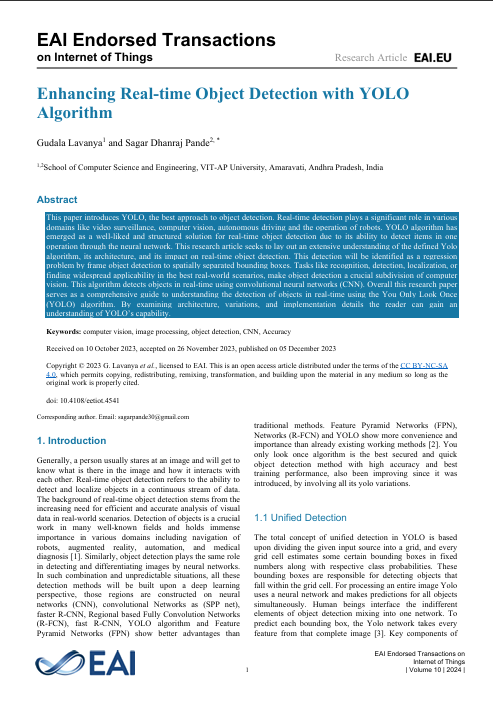
\includegraphics[width=0.8\textwidth]{reference_papers/Paper_1.png}
    % Includes an image of Paper 1 from the 'reference_papers' folder.
    % The image is scaled to 80% of the text width (0.8\textwidth).
\end{figure}
% Ends the figure environment for Paper 1.
%
%
% Paper 2
\\\\
% Inserts two line breaks before Paper 2.
\textbf{[B2.]}
% Displays "B2." in bold to represent the second reference paper.
%
%
%
\begin{figure}[h!]
    \centering
    % Centers the figure on the page.
    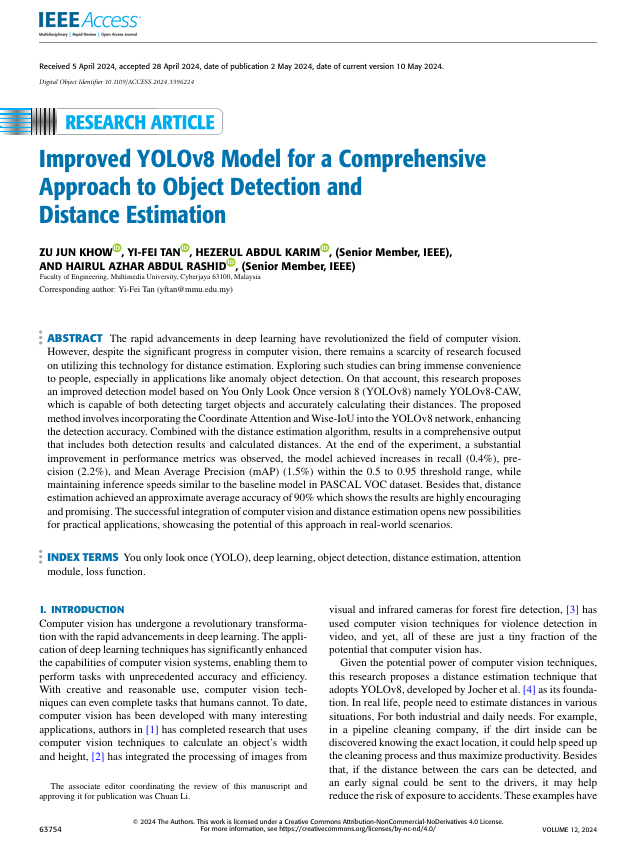
\includegraphics[width=1\textwidth]{reference_papers/Paper_2(Base Paper).png}
    % Includes an image of Paper 2 (Base Paper) from the 'reference_papers' folder.
    % The image is scaled to the full width of the text area (1\textwidth).
\end{figure}
% Ends the figure environment for Paper 2.
%
%
% Paper 3
\\\\\\\\
% Inserts four line breaks before Paper 3.
\textbf{[B3.]}
% Displays "B3." in bold to represent the third reference paper.
%
%
%
\begin{figure}[h!]
    \centering
    % Centers the figure on the page.
    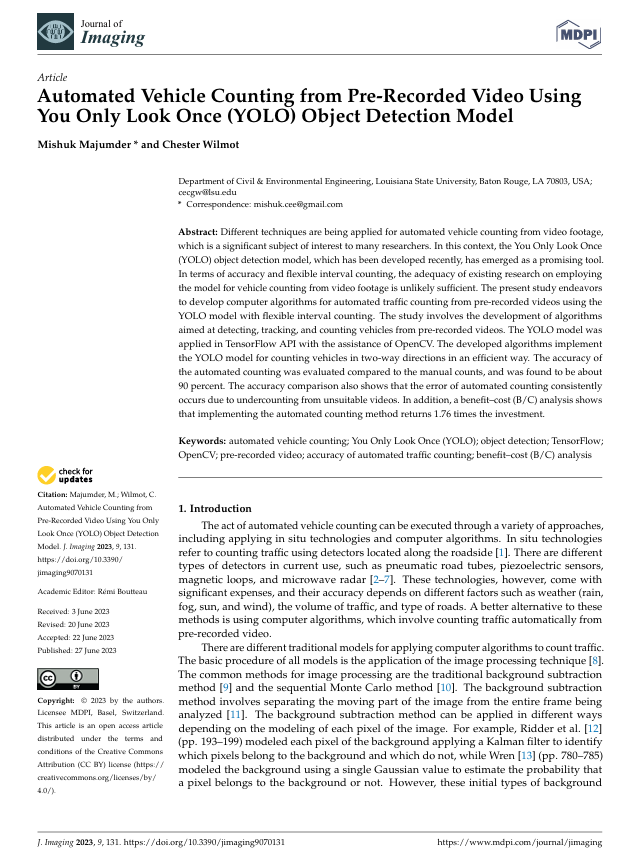
\includegraphics[width=1\textwidth]{reference_papers/Paper_3.png}
    % Includes an image of Paper 3 from the 'reference_papers' folder.
    % The image is scaled to the full width of the text area (1\textwidth).
\end{figure}
% Ends the figure environment for Paper 3.
%
%
% Paper 4
\\\\\\\\
% Inserts two line breaks before Paper 4.
\textbf{[B4.]}
% Displays "B4." in bold to represent the fourth reference paper.
%
%
%
\begin{figure}[h!]
    \centering
    % Centers the figure on the page.
    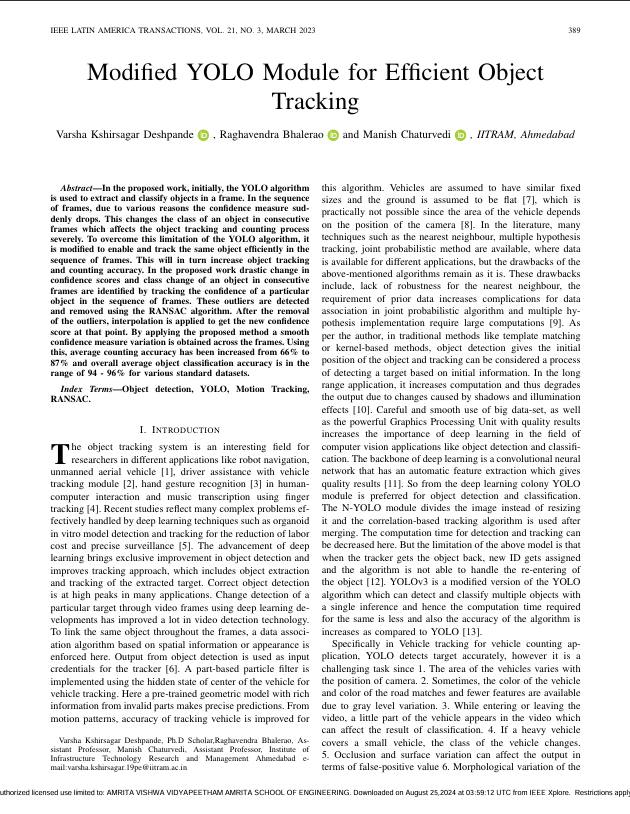
\includegraphics[width=1\textwidth]{reference_papers/Paper_4.png}
    % Includes an image of Paper 4 from the 'reference_papers' folder.
    % The image is scaled to the full width of the text area (1\textwidth).
\end{figure}
% Ends the figure environment for Paper 4.
%
% End of the chapter
%
%
% Includes Appendix B.

% Appendix C Page
\prefacesection{Appendix C: Viva Q\&A}
% Creates a section titled "Appendix C: Viva Q&A" for displaying the viva questions and answers.
%
%
%
\textbf{Q: What is the main advantage of the YOLO (You Only Look Once) algorithm for object detection?} \\
% Bold text for the first question.
A: The main advantage of the YOLO algorithm is its ability to perform real-time object detection with high accuracy. YOLO treats object detection as a single-stage problem, predicting both bounding boxes and class probabilities in one evaluation, which makes it significantly faster than traditional methods like R-CNN.
% Answer to the first question explaining the efficiency and speed of YOLO over traditional methods.
\\\\
% Inserts two line breaks for spacing.
%
%
\textbf{Q: What is non-maximum suppression (NMS) in the context of the YOLO algorithm?} \\
% Bold text for the second question.
A: Non-maximum suppression (NMS) is a technique used in YOLO to eliminate duplicate bounding box predictions for the same object. It involves selecting the bounding box with the highest confidence score, computing the Intersection over Union (IoU) with other boxes of the same class, and removing boxes with an IoU greater than a specified threshold.
% Answer to the second question explaining how NMS reduces redundant bounding boxes for the same object.
\\\\
% Inserts two line breaks for spacing.
%
%
\textbf{Q: How does the YOLOv8-CAW model improve object detection accuracy?} \\
% Bold text for the third question.
A: The YOLOv8-CAW model improves object detection accuracy by integrating the Coordinate Attention (CA) module and the Wise-IoU loss function. The CA module enhances the model's focus on important regions of the image, while the Wise-IoU loss function improves bounding box predictions by adjusting loss coefficients based on the quality of samples.
% Answer to the third question explaining the improvements in YOLOv8-CAW model through the use of CA and Wise-IoU loss function.
%
% End of the chapter
%
%
% Includes Appendix C.

\end{document}
%
% End of the document
%
%